% Chapter Template
\chapter{Results} % Main chapter title

\label{Results} % Change X to a consecutive number; for referencing this chapter elsewhere, use \ref{ChapterX}

This chapter presents findings from the experiments conducted to evaluate Sarosh’s Perceptron Networks (SPNs) against traditional Multi-Layer Perceptrons (MLPs), addressing the research questions outlined in Chapter \ref{Introduction}. The results are organized into three sections corresponding to the domains evaluated: Images, Tabular Data, and Text Data. For each domain, results from all model architectures detailed in Chapter \ref{Experiments} are presented, compared, and analyzed.

Throughout this chapter, shorter representations for model names and evaluations have been adopted for clarity:

\begin{table}[h!]
    \centering
    \begin{tabular}{ll}
    \textbf{Full name} & \textbf{Representation used} \\
    \hline
    Models: & \\
    \hspace{1em} Baseline MLP & base\_mlp \\
    \hspace{1em} Free Weights SPN & fw\_spn \\
    \hspace{1em} Minimal SPN & min\_spn \\
    \hspace{1em} Minimal MLP & min\_mlp \\
    \hspace{1em} Maximal SPN & max\_spn \\
    \hspace{1em} Pruned Maximal SPN & pruned\_spn \\
    Evaluation Metrics: & \\
    \hspace{1em} Parameter Count & param\_count \\
    \hspace{1em} Best Test Accuracy & best\_acc \\
    \hspace{1em} Time to Best Accuracy & time\_best \\
    \hspace{1em} Training Efficiency & train\_eff \\
    \hspace{1em} Area Under Curve Efficiency & auc\_eff \\
    \hspace{1em} Throughput Efficiency & thru\_eff \\
    \end{tabular}
\end{table}

%----------------------------------------------------------------------------------------
%	SECTION 1
%----------------------------------------------------------------------------------------

\section{Image Domain Results}

Both image datasets were flattened and normalized before model training.

\subsection{MNIST Dataset}

\begin{tabular}{@{}ll@{}}
\textbf{Variant} & Simple \\
\textbf{Input Features} & 784 \\
\textbf{Output Classes} & 10 \\
\textbf{Batch Size} & 75 \\
\textbf{Training Epochs} & 50 \\
\textbf{Training Samples} & 60,000 \\
\textbf{Test Samples} & 10,000 \\
\textbf{Base MLP Dimensions} & $[12,\, 12,\, 10]$ \\
\textbf{Total Neurons} & 34 \\
\end{tabular}

\begin{figure}[H]
    \centering
    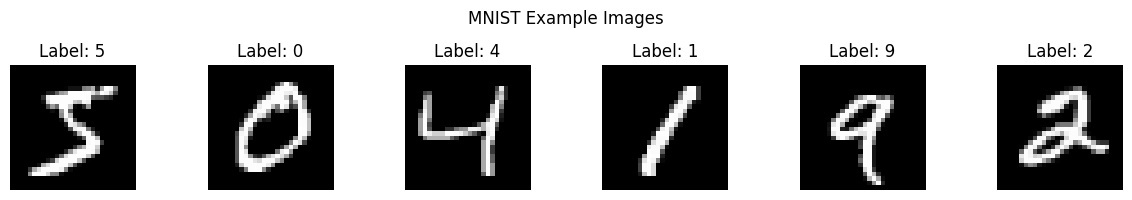
\includegraphics[width=1.0\textwidth]{Figures/Results/MNIST/examples.png} 
    \captionsetup{justification=centering}  % Ensure the caption is centered
    \caption{Example Images in MNIST}
    \label{fig:mnistexamples}
\end{figure}

Preliminary testing showed that very large MLP models could achieve test accuracies approaching those of state-of-the-art models reported on the MNIST leaderboard~\cite{pwc_mnist_leaderboard}, with results nearing 98\%. However, at this level of performance, any improvements offered by SPNs would likely be marginal and difficult to observe. For this reason, a smaller model was chosen as the base MLP to make potential improvements more evident.

\begin{figure}[H]
    \centering
    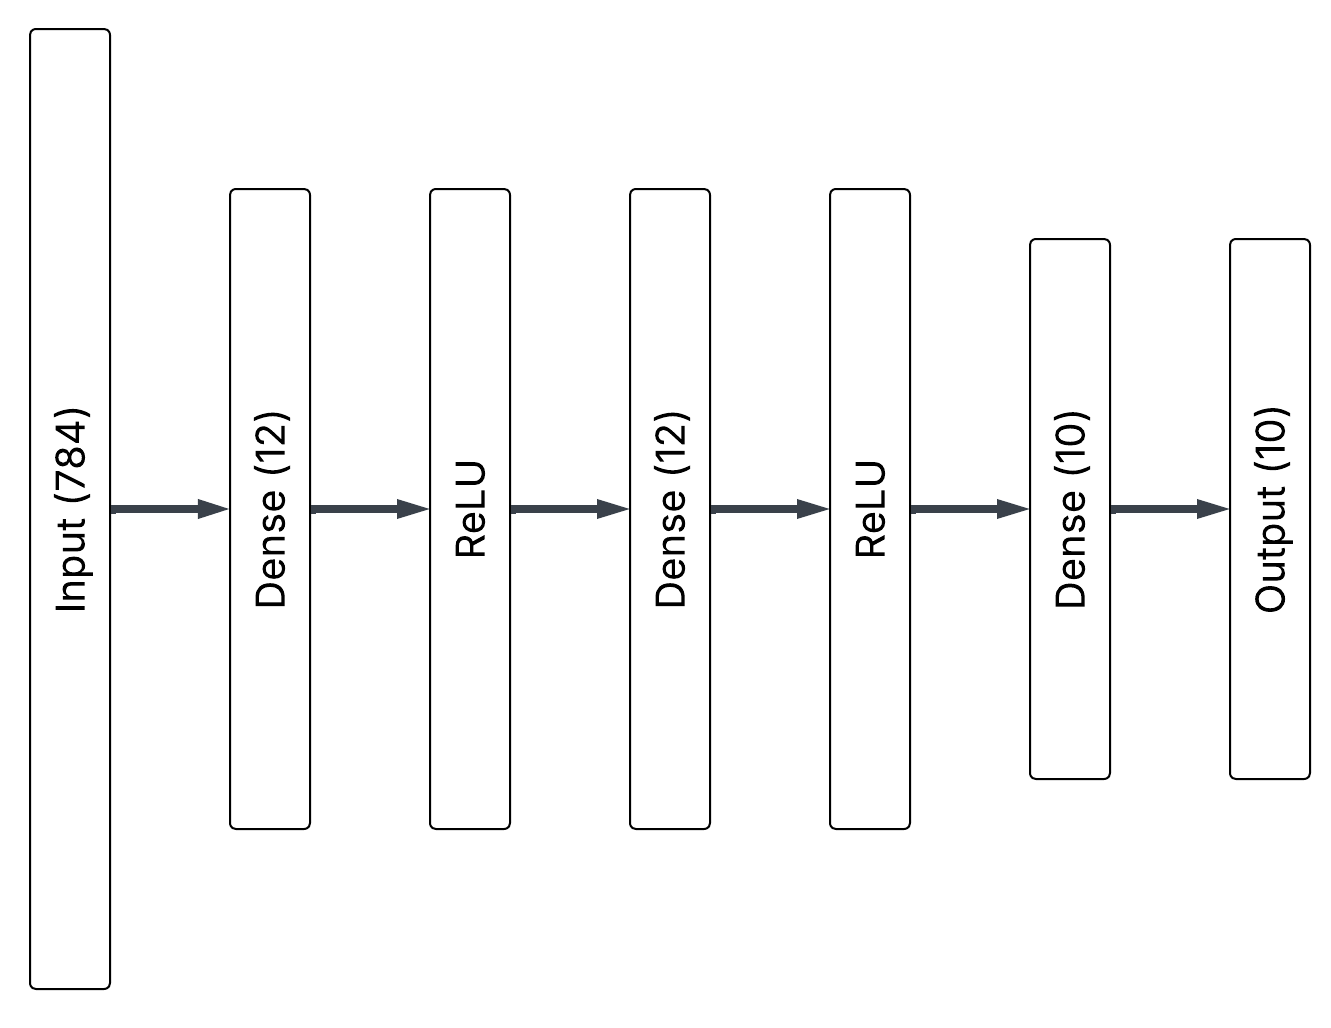
\includegraphics[width=0.6\textwidth]{Figures/Results/MNIST/MNIST_base_mlp_architecture.png} 
    \captionsetup{justification=centering}  % Ensure the caption is centered
    \caption{base\_mlp architecture for MNIST}
    \label{fig:mnistMlpBaseArch}
\end{figure}

The training and testing curves in Figures \ref{fig:mnistTrainCurve} and \ref{fig:mnistTestCurve} clearly demonstrate that the min\_mlp and base\_mlp models underperform relative to all SPN models. Table \ref{tab:mnistResults} offers a detailed comparison of all six models across the efficiency metrics.

\begin{figure}[H]
    \centering
    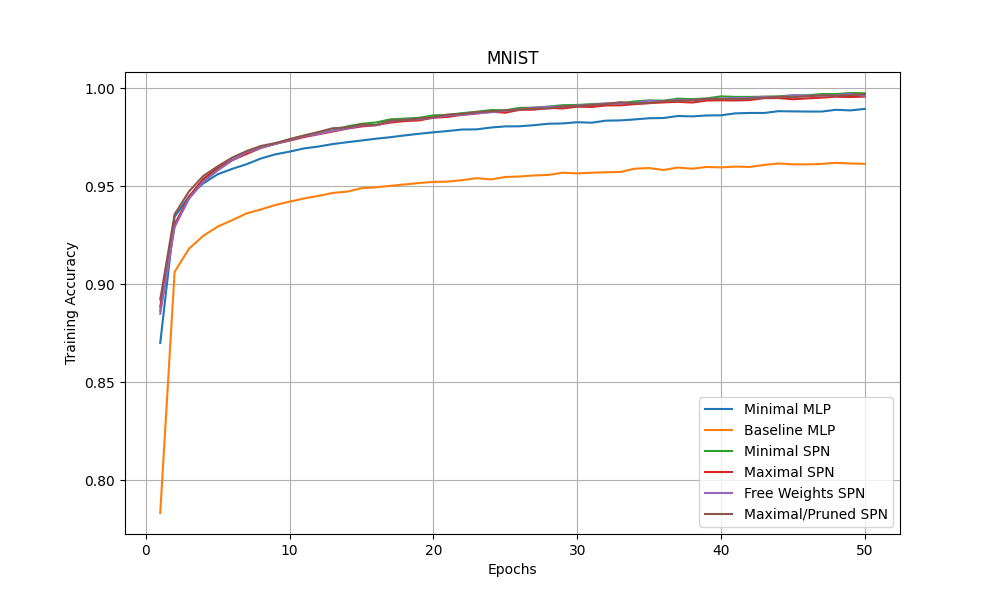
\includegraphics[width=\linewidth]{Figures/Results/MNIST/training_accuracy_plot.png} % first figure itself
    \captionsetup{width=\linewidth}
    \caption{train\_acc vs epochs curve for MNIST}
    \label{fig:mnistTrainCurve}
\end{figure}

\begin{figure}[H]
    \centering
    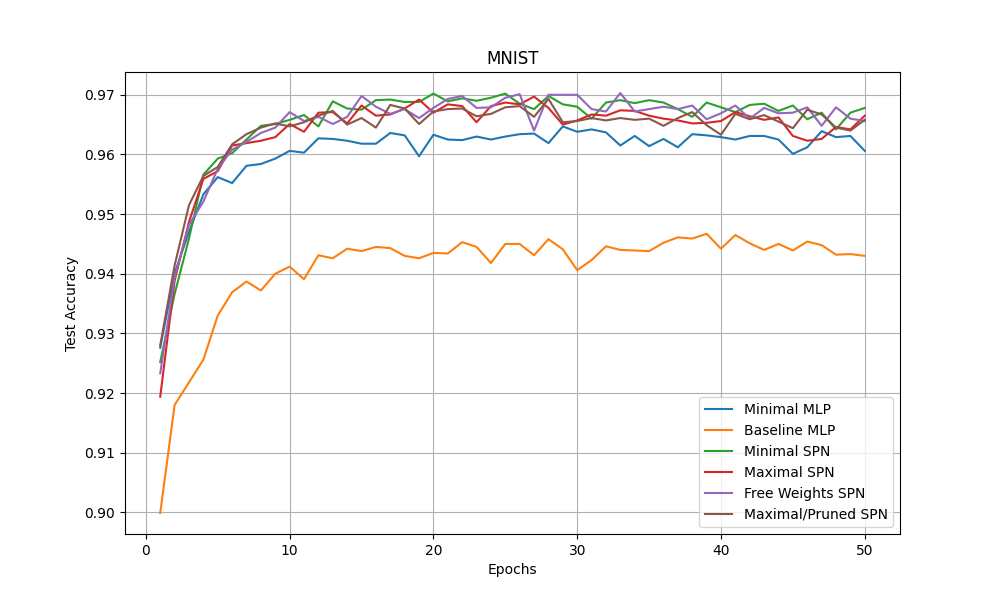
\includegraphics[width=\linewidth]{Figures/Results/MNIST/test_accuracy_plot.png} % second figure itself
    \captionsetup{width=\linewidth}
    \caption{test\_acc vs epochs curve for MNIST}
    \label{fig:mnistTestCurve}
\end{figure}

\begin{table}[h!]
    \centering
    \caption{Cross Model Comparison on the MNIST dataset}
    \begin{tabular}{|l|l|l|l|l|l|l|}
    \hline
    \textbf{Model} & \textbf{param\_count} & \textbf{best\_acc} & \textbf{time\_best} & \textbf{train\_eff} & \textbf{auc\_eff} & \textbf{thru\_eff} \\
    \hline
    base\_mlp & 9,706 & \cellcolor{red!25}94.67\% & 45.34s & 0.021 & \cellcolor{red!25}46.131 & 0.816 \\
    fw\_spn & 27,074  & \cellcolor{green!25}97.03\% & 53.09s  & 0.018 & 47.297 & 0.607 \\
    min\_mlp & 19,090 & 96.47\% & 24.85s & 0.039 & 47.074 & \cellcolor{green!25}1.127 \\
    min\_spn & 26,930 & 97.02\% & \cellcolor{green!25}18.23  & \cellcolor{green!25}0.053 & \cellcolor{green!25}47.318 & 1.043 \\
    max\_spn & 27,251  & 96.97\% & \cellcolor{red!25}399.87s & \cellcolor{red!25}0.002 & 47.246 & \cellcolor{red!25}0.064 \\
    pruned\_spn & 27,025 & 96.93\% & 44.99s & 0.022 & 47.256 & 0.595 \\
    \hline
    \end{tabular}
    \label{tab:mnistResults}
\end{table}

\begin{enumerate}
\item \textbf{Baseline MLP vs. Free Weights SPN}: The fw\_spn model achieved the highest test accuracy, clearly outperforming the base\_mlp, which had the lowest accuracy out of all the models. The notable increase in parameter count of the fw\_spn, while retaining the same layer layout as the base\_mlp, correlates positively with its improved accuracy, providing strong evidence that enhanced internal connectivity boosts model performance. Although fw\_spn had slightly lower training and throughput efficiencies than the base\_mlp, this trade-off was justified by the considerable gain in accuracy.
\item \textbf{Minimal MLP vs. Minimal SPN}: Both min\_spn and min\_mlp achieved better accuracy compared to base\_mlp but slightly lower than fw\_spn. This suggests that having a higher param\_count might be more advantageous in this dataset than having more layers. Min\_spn consistently outperformed min\_mlp across all metrics except throughput efficiency, where both models were fairly close to one another. This further emphasizes the benefit of increased neural connectivity on model performance.
\item \textbf{Maximal SPN}: Max\_spn model had the third-highest accuracy but required significantly longer training times compared to the other models. This suggests a performance ceiling for the MNIST dataset, where additional internal connections yield diminishing returns.
\item \textbf{Pruned SPN}:
\begin{center}  % Centers the table
\begin{tabular}{|l|l|}
\hline
\textbf{Metric} & \textbf{Value} \\
\hline
Layers Before Pruning & 34 \\
Layers After Pruning & 3 \\
Mean Epoch Time Before Pruning & 15.89s \\
Mean Epoch Time After Pruning & 1.59s \\
Pruning Time & 631.68s \\
Pruning Effectiveness & 9.99 \\
\hline
\end{tabular}
\end{center}

The pruned\_spn model achieved accuracy similar to max\_spn while dramatically improving computational efficiency. Although the pruning process itself was time-consuming, taking longer than it took max\_spn to reach its peak accuracy (making it practically unusable), it still made the max\_spn model nearly 10x faster in average training time, validating the efficacy of pruning for optimizing maximal SPNs. Additionally, this pruning confirmed that a three-layer architecture is sufficient for optimal performance on this dataset. 

However, since max\_spn did not outperform any of the other models, it suggests that there was limited additional learning to be done, making pruning easier on this particular dataset.
\end{enumerate}

Overall, SPNs convincingly outperformed their MLP counterparts on the MNIST dataset. Maximal and pruned SPNs confirmed the existence of an upper performance bound, highlighting the effectiveness of strategic pruning to balance accuracy and efficiency.

\subsection{CIFAR 10 Dataset}

\begin{tabular}{@{}ll@{}}
\textbf{Variant} & Complex \\
\textbf{Input Features} & 3072 \\
\textbf{Output Classes} & 10 \\
\textbf{Batch Size} & 128 \\
\textbf{Training Epochs} & 30 \\
\textbf{Training Samples} & 50,000 \\
\textbf{Test Samples} & 10,000 \\
\textbf{Base MLP Dimensions} & $[256,\, 128,\, 64,\, 32,\, 10]$ \\
\textbf{Total Neurons} & 490 \\
\end{tabular}

\begin{figure}[H]
    \centering
    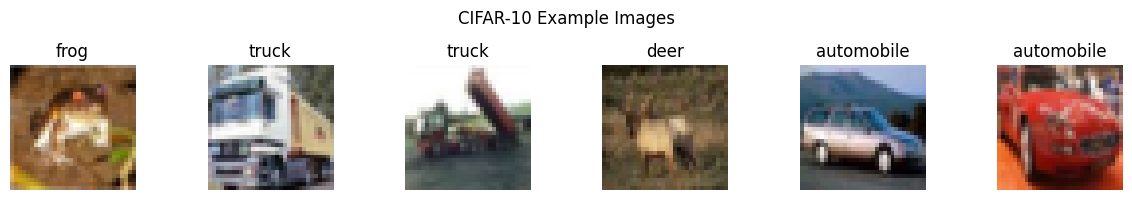
\includegraphics[width=1.0\textwidth]{Figures/Results/CIFAR_10/examples.png} 
    \captionsetup{justification=centering}  % Ensure the caption is centered
    \caption{Example Images in CIFAR 10}
    \label{fig:cifarexamples}
\end{figure}

In preliminary tests on this dataset, all MLP models exhibited clear overfitting. This contrasted with the results on MNIST, likely because MNIST images are much simpler (being grayscale handwritten digits) \ref{fig:mnistexamples}, and the train and test sets are more homogeneous. In CIFAR-10, however, the diversity and complexity of classes \ref{fig:cifarexamples}, as well as the substantial differences between training and test samples, pose challenges that perceptron-based models struggle to overcome. This aligns with observations from the CIFAR-10 leaderboard~\cite{pwc_cifar10_leaderboard}, where the best-performing models are specialized architectures such as Convolutional Neural Networks (CNNs) and Vision Transformers (ViTs).

Although data augmentation and regularization techniques were applied in initial experiments, they did not yield significant improvements. Consequently, this dataset was used to illustrate the upper limits of complexity in image classification and to examine how MLPs and SPNs (both based on perceptron architectures) compare when faced with such challenging data. This dataset also had the largest base\_mlp model among all datasets used in these experiments.

\begin{figure}[H]
    \centering
    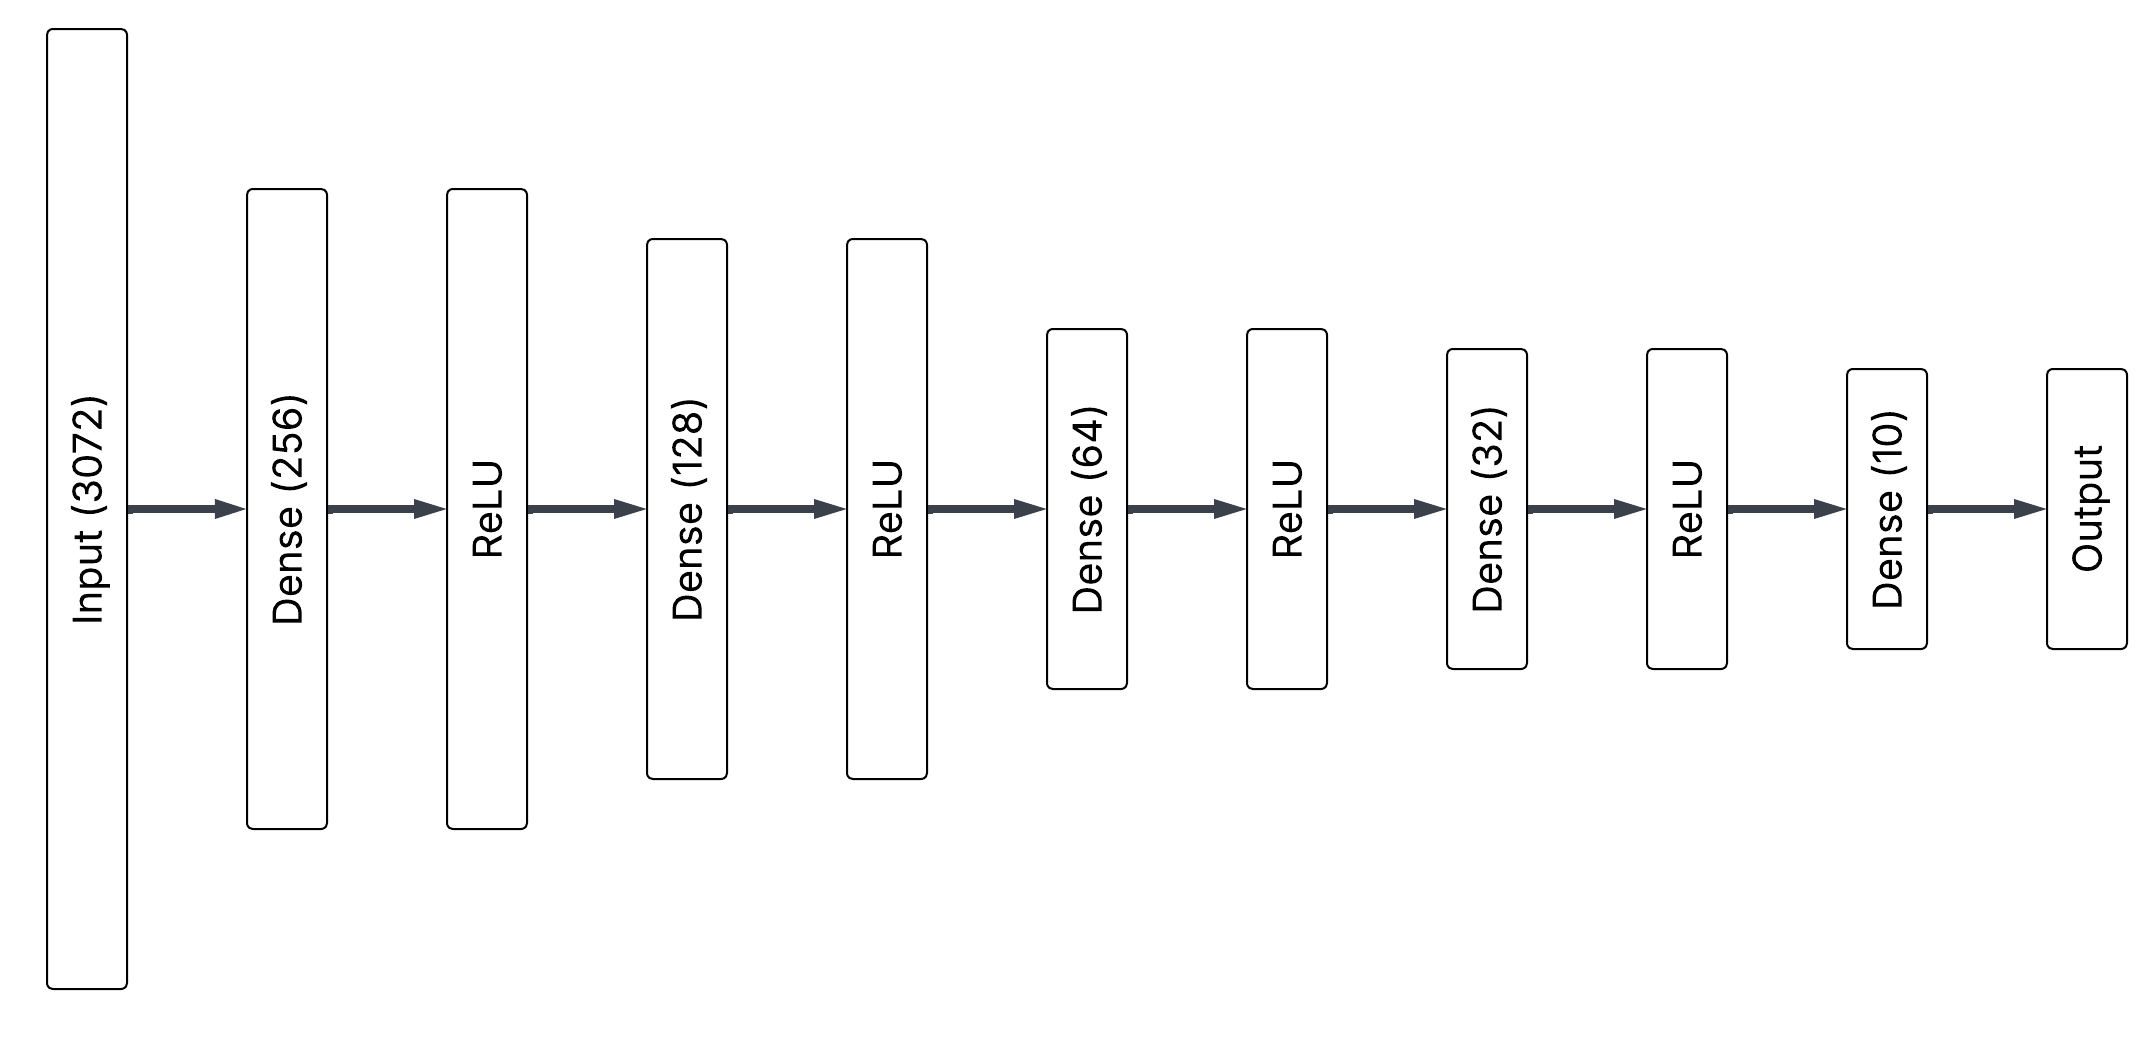
\includegraphics[width=1.0\textwidth]{Figures/Results/CIFAR_10/CIFAR_base_mlp_architecture.png} 
    \captionsetup{justification=centering}  % Ensure the caption is centered
    \caption{base\_mlp architecture for CIFAR 10}
    \label{fig:cifarMlpBaseArch}
\end{figure}

The training curve in Figure \ref{fig:cifarTrainCurve} follows the expected trend: the smaller models (min\_mlp and min\_spn) underperform relative to base\_mlp and fw\_spn, while pruned\_spn and max\_spn achieve the highest training scores. However, the test curve in Figure \ref{fig:cifarTestCurve} reveals that base\_mlp outperforms all other models on unseen data. This indicates that increasing the number of connections may actually worsen generalization in this case, as it encourages overfitting to the training set. Table \ref{tab:cifarResults} provides additional evidence to support this observation.

\begin{figure}[H]
    \centering
    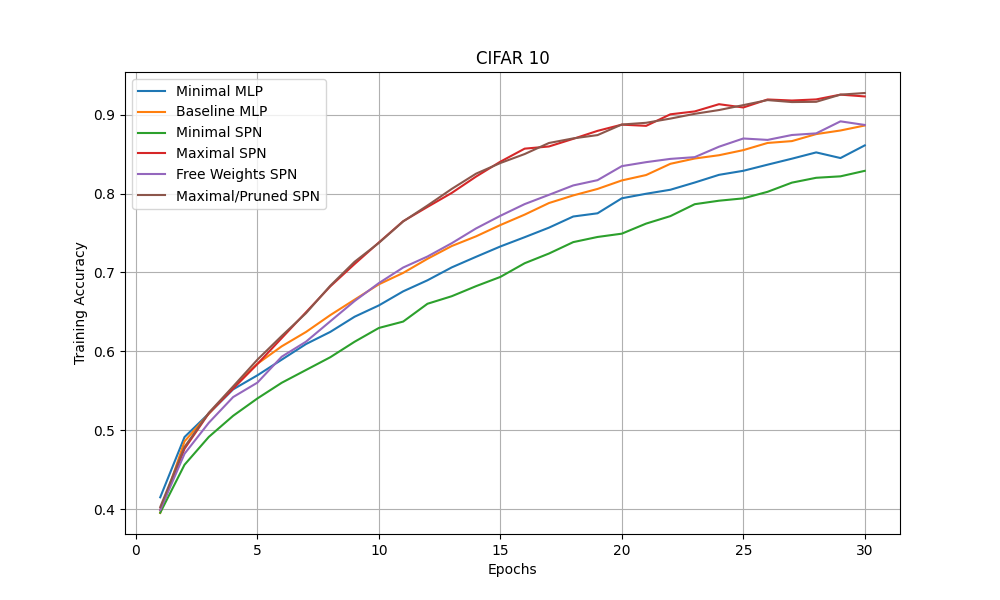
\includegraphics[width=\linewidth]{Figures/Results/CIFAR_10/training_accuracy_plot.png} % first figure itself
    \captionsetup{width=\linewidth}
    \caption{train\_acc vs epochs curve for CIFAR 10}
    \label{fig:cifarTrainCurve}
\end{figure}

\begin{figure}[H]
    \centering
    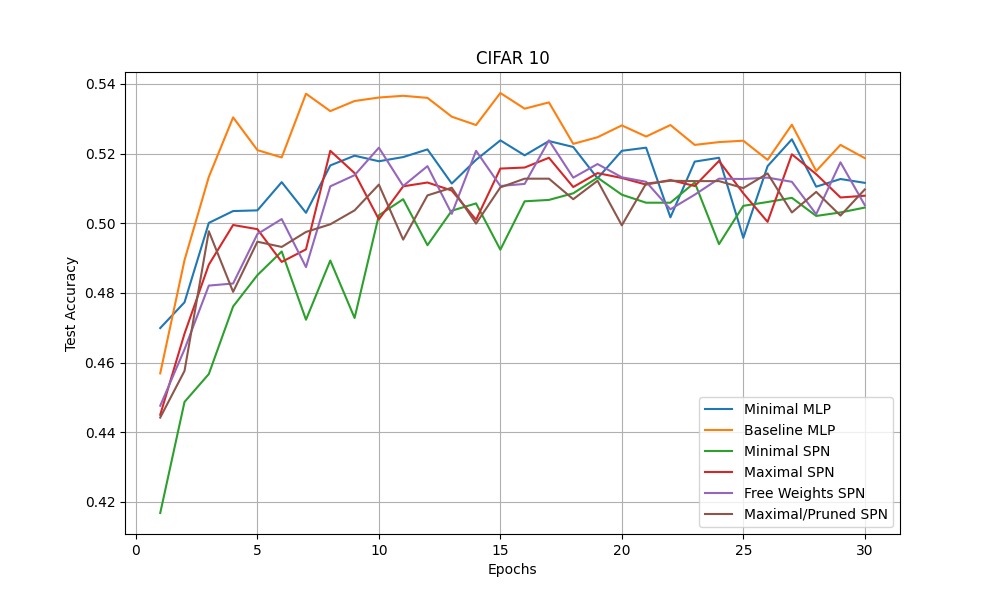
\includegraphics[width=\linewidth]{Figures/Results/CIFAR_10/test_accuracy_plot.png} % second figure itself
    \captionsetup{width=\linewidth}
    \caption{test\_acc vs epochs curve for CIFAR 10}
    \label{fig:cifarTestCurve}
\end{figure}

\begin{table}[h!]
    \centering
    \caption{Cross Model Comparison on the CIFAR 10 Dataset}
    \begin{tabular}{|l|l|l|l|l|l|l|}
    \hline
    \textbf{Model} & \textbf{param\_count} & \textbf{best\_acc} & \textbf{time\_best} & \textbf{train\_eff} & \textbf{auc\_eff} & \textbf{thru\_eff} \\
    \hline
    base\_mlp & 830,250 & \cellcolor{green!25}53.74\% & 14.12s & 0.038 & \cellcolor{green!25}15.220 & 0.585 \\
    fw\_spn & 1,582,250 & 52.38\% & 19.57s & 0.027 & 14.671 & 0.449 \\
    min\_mlp & 1,479,850 & 52.41\% & 12.83s & 0.041 & 14.856 & \cellcolor{green!25}1.100 \\
    min\_spn & 1,510,570 & \cellcolor{red!25}51.31\% & \cellcolor{green!25}10.60s & \cellcolor{green!25}0.048 & \cellcolor{red!25}14.342 & 0.925 \\
    max\_spn & 1,625,575 & 52.08\% & \cellcolor{red!25}472.26s & \cellcolor{red!25}0.001 & 14.672 & \cellcolor{red!25}0.009 \\
    pruned\_spn & 1,623,931 & 51.43\% & 453.08s & \cellcolor{red!25}0.001 & 14.567 & 0.029 \\
    \hline
    \end{tabular}
    \label{tab:cifarResults}
\end{table}

\begin{enumerate}
\item \textbf{Baseline MLP vs. Free Weights SPN}: The base\_mlp achieved the highest test accuracy, with the fw\_spn following closely behind. Additionally, base\_mlp demonstrated greater efficiency than fw\_spn, further underscoring the limitations of increasing internal connectivity in perceptron-based models. In complex datasets like CIFAR 10, where spatial relationships are lost during flattening, increasing connections primarily leads to greater overfitting rather than better generalization, making the less-connected base\_mlp the better choice.
\item \textbf{Minimal MLP vs. Minimal SPN}: A similar trend was observed with the smaller models, min\_mlp attained the second-highest test accuracy and overall efficiency, while min\_spn recorded the lowest test accuracy. This further supports the conclusion that, in scenarios prone to overfitting, additional connections can degrade model performance.
\item \textbf{Maximal SPN}: The max\_spn model achieved only moderate test accuracy, indicating that increasing model depth or complexity does not translate to improved results for perceptron-based models on CIFAR-10. This suggests that such architectures are inherently limited in capturing the complex relationships present in image data.
\item \textbf{Pruned SPN}:
\begin{center}  % Centers the table
\begin{tabular}{|l|l|}
\hline
\textbf{Metric} & \textbf{Value} \\
\hline
Layers Before Pruning & 34 \\
Layers After Pruning & 86 \\
Mean Epoch Time Before Pruning & 62.06s \\
Mean Epoch Time After Pruning & 17.85s \\
Pruning Time & 1520.61s \\
Pruning Effectiveness & 3.48 \\
\hline
\end{tabular}
\end{center}

Although the pruned\_spn improved the throughput of max\_spn, it did not offer meaningful gains in training or AUC efficiency. Since max\_spn itself was not a strong performer, improving its speed offers little practical value. Moreover, the pruning process took significantly longer than the best\_time for max\_spn, highlighting inefficiencies in the pruning algorithm and the need for further optimization.

\end{enumerate}

Overall, this experiment highlighted the limitations of perceptron-based models when applied to complex image data. SPNs did not provide any meaningful improvements on such datasets; in fact, their increased internal connectivity exacerbated the overfitting already observed in traditional MLPs, ultimately leading to even poorer generalization performance.

\section{Tabular Domain Results}

For these datasets, pre-processing involved filling missing values, encoding categorical variables and removing unncessary features.

\subsection{Titanic Dataset}

\begin{tabular}{@{}ll@{}}
\textbf{Variant} & Simple \\
\textbf{Input Features} & 7 \\
\textbf{Output Classes} & 2 \\
\textbf{Batch Size} & 32 \\
\textbf{Training Epochs} & 50 \\
\textbf{Training Samples} & 712 \\
\textbf{Test Samples} & 179 \\
\textbf{Base MLP Dimensions} & $[16,\, 8,\, 4,\, 2]$ \\
\textbf{Total Neurons} & 30 \\
\end{tabular}

\vspace{2pt}

During pre-processing, missing values in the 'Age' and 'Embarked' fields were imputed using the median age and the most frequent embarkation point, respectively. The 'Sex' field was converted to a binary variable, while the 'Embarked' field was encoded numerically. The 'Name', 'Ticket', 'Cabin', and 'PassengerId' fields were removed, as they were not relevant for predicting passenger survival. Finally, the 'Survived' column was separated as the target variable.

In early testing, MLP models of various sizes exhibited similar test performance, suggesting that the dataset’s information content may be limited and not further exploitable by increasing model size, especially given the small training set. Consequently, a compact base\_mlp model was chosen to represent traditional MLP performance on such small datasets.

\begin{figure}[H]
    \centering
    \includegraphics[height=0.28\textheight,width=0.7\textwidth]{Figures/Results/Titanic/titanic_base_mlp_architecture.png} 
    \captionsetup{justification=centering}  % Ensure the caption is centered
    \caption{base\_mlp architecture for Titanic}
    \label{fig:titanicMlpBaseArch}
\end{figure}

The training and test curves in Figures \ref{fig:titanicTrainCurve} and \ref{fig:titanicTestCurve} indicate that all models quickly converge to their optimal performance, with no single model standing out as clearly superior or inferior. Given that the best accuracy achieved across all six models in table \ref{tab:titanicResults} is one of two values, and the small sizes of both the training and test sets, this strongly suggests that additional data would be necessary to capture any subtle patterns within the dataset, and that increasing model connectivity through SPNs alone offers little benefit in this context.

\begin{figure}[H]
    \centering
    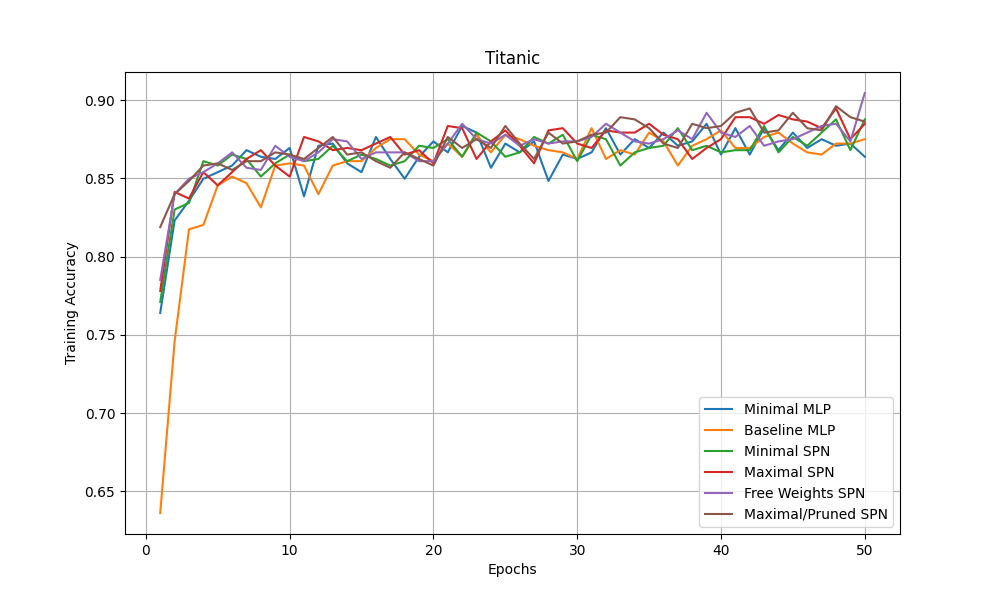
\includegraphics[width=\linewidth]{Figures/Results/Titanic/training_accuracy_plot.png} % first figure itself
    \captionsetup{width=\linewidth}
    \caption{train\_acc vs epochs curve for Titanic}
    \label{fig:titanicTrainCurve}
\end{figure}

\begin{figure}[H]
    \centering
    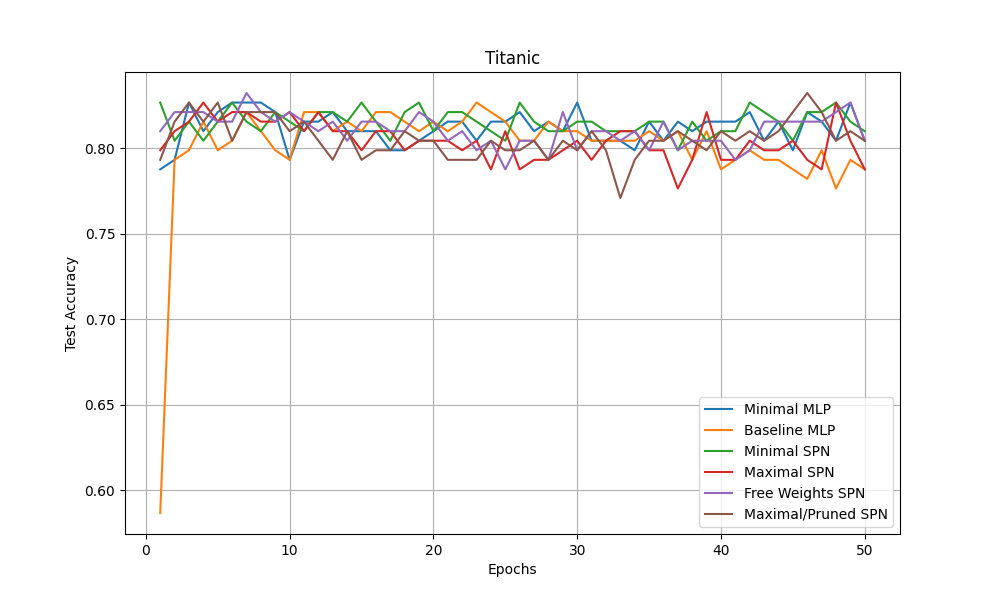
\includegraphics[width=\linewidth]{Figures/Results/Titanic/test_accuracy_plot.png} % second figure itself
    \captionsetup{width=\linewidth}
    \caption{test\_acc vs epochs curve for Titanic}
    \label{fig:titanicTestCurve}
\end{figure}

\begin{table}[h!]
    \centering
    \caption{Titanic Dataset results}
    \begin{tabular}{|l|l|l|l|l|l|l|}
    \hline
    \textbf{Model} & \textbf{param\_count} & \textbf{best\_acc} & \textbf{time\_best} & \textbf{train\_eff} & \textbf{auc\_eff} & \textbf{thru\_eff} \\
    \hline
    base\_mlp & 310 & \cellcolor{red!25}82.68\% & 0.86s & 0.960 & \cellcolor{red!25}39.369 & 22.032 \\
    fw\_spn & 520 & \cellcolor{green!25}83.24\% & 0.33s & 2.560 & 39.735 & 18.331 \\
    min\_mlp & 282 & \cellcolor{red!25}82.68\% & 0.09s & 9.020 & 39.802 & \cellcolor{green!25}36.282 \\
    min\_spn & 296 & \cellcolor{red!25}82.68\% & \cellcolor{green!25}0.02s & \cellcolor{green!25}34.747 & \cellcolor{green!25}39.941 & 33.714 \\
    max\_spn & 675 & \cellcolor{red!25}82.68\% & 1.72s & 0.482 & 39.430 & \cellcolor{red!25}2.376 \\
    pruned\_spn & 655 & \cellcolor{green!25}83.24\% & \cellcolor{red!25}8.05s & \cellcolor{red!25}0.103 & 39.503 & 4.746 \\
    \hline
    \end{tabular}
    \label{tab:titanicResults}
\end{table}

\begin{enumerate}
\item \textbf{Baseline MLP vs. Free Weights SPN}: Although all models performed similarly overall, the fw\_spn outperformed the base\_mlp in every metric except throughput efficiency. However, the slight reduction in throughput is easily justified by the fw\_spn’s higher accuracy, as well as its significantly better training efficiency and AUC efficiency scores.
\item \textbf{Minimal MLP vs. Minimal SPN}: While both small models achieved similar test accuracy, the min\_spn surpassed the min\_mlp and all other models in training efficiency. Although min\_mlp demonstrated higher throughput efficiency, potentially making it more suitable for practical deployment, the superior training and AUC efficiency of min\_spn make it a preferable choice for evaluating performance on small datasets for testing and research purposes.
\item \textbf{Maximal SPN}: As with the MNIST and CIFAR-10 datasets, the max\_spn did not demonstrate any significant performance gains and exhibited poor efficiency scores. This further highlights that increasing the layer count in perceptron-based models yields little to no benefit, particularly when working with small datasets.
\item \textbf{Pruned SPN}:
\begin{center}  % Centers the table
\begin{tabular}{|l|l|}
\hline
\textbf{Metric} & \textbf{Value} \\
\hline
Layers Before Pruning & 30 \\
Layers After Pruning & 15 \\
Mean Epoch Time Before Pruning & 0.32s \\
Mean Epoch Time After Pruning & 0.18s \\
Pruning Time & 1.65s \\
Pruning Effectiveness & 1.78 \\
\hline
\end{tabular}
\end{center}
The pruned\_spn was arguably the weakest performer in this test, recording the lowest training efficiency and the worst time to best test accuracy. Moreover, the pruning process took as long as it did for max\_spn to reach its best accuracy. Altogether, these results indicate that pruning offered no meaningful benefit for such a small dataset.

\end{enumerate}

Overall, the small dataset size limited our ability to observe strong evidence that increased connectivity improves performance on tabular data. However, the fact that the SPN counterparts consistently outperformed their MLP equivalents provides a promising indication of the potential benefits of enhanced connectivity.

\subsection{Covertype Dataset}

\begin{tabular}{@{}ll@{}}
\textbf{Variant} & Complex \\
\textbf{Input Features} & 54 \\
\textbf{Output Classes} & 7 \\
\textbf{Batch Size} & 256 \\
\textbf{Training Epochs} & 150 \\
\textbf{Training Samples} & 88,314 \\
\textbf{Test Samples} & 22,079 \\
\textbf{Base MLP Dimensions} & $[128,\, 64,\, 7]$ \\
\textbf{Total Neurons} & 199 \\
\end{tabular}

For preprocessing, the numeric columns were normalized, and the categorical features for soil types 1–40 were encoded as binary variables.

Early testing revealed that bigger MLPs achieved competitive accuracy on this dataset, comparable to the results reported on the leaderboards~\cite{kaggle_covertype_leaderboard}. And since the test accuracy was closer to 80\%, a three-layer MLP of substantial size was selected for further experiments as there was signifcant room for observing improvements, if any were made by using SPN techniques.

\begin{figure}[H]
    \centering
    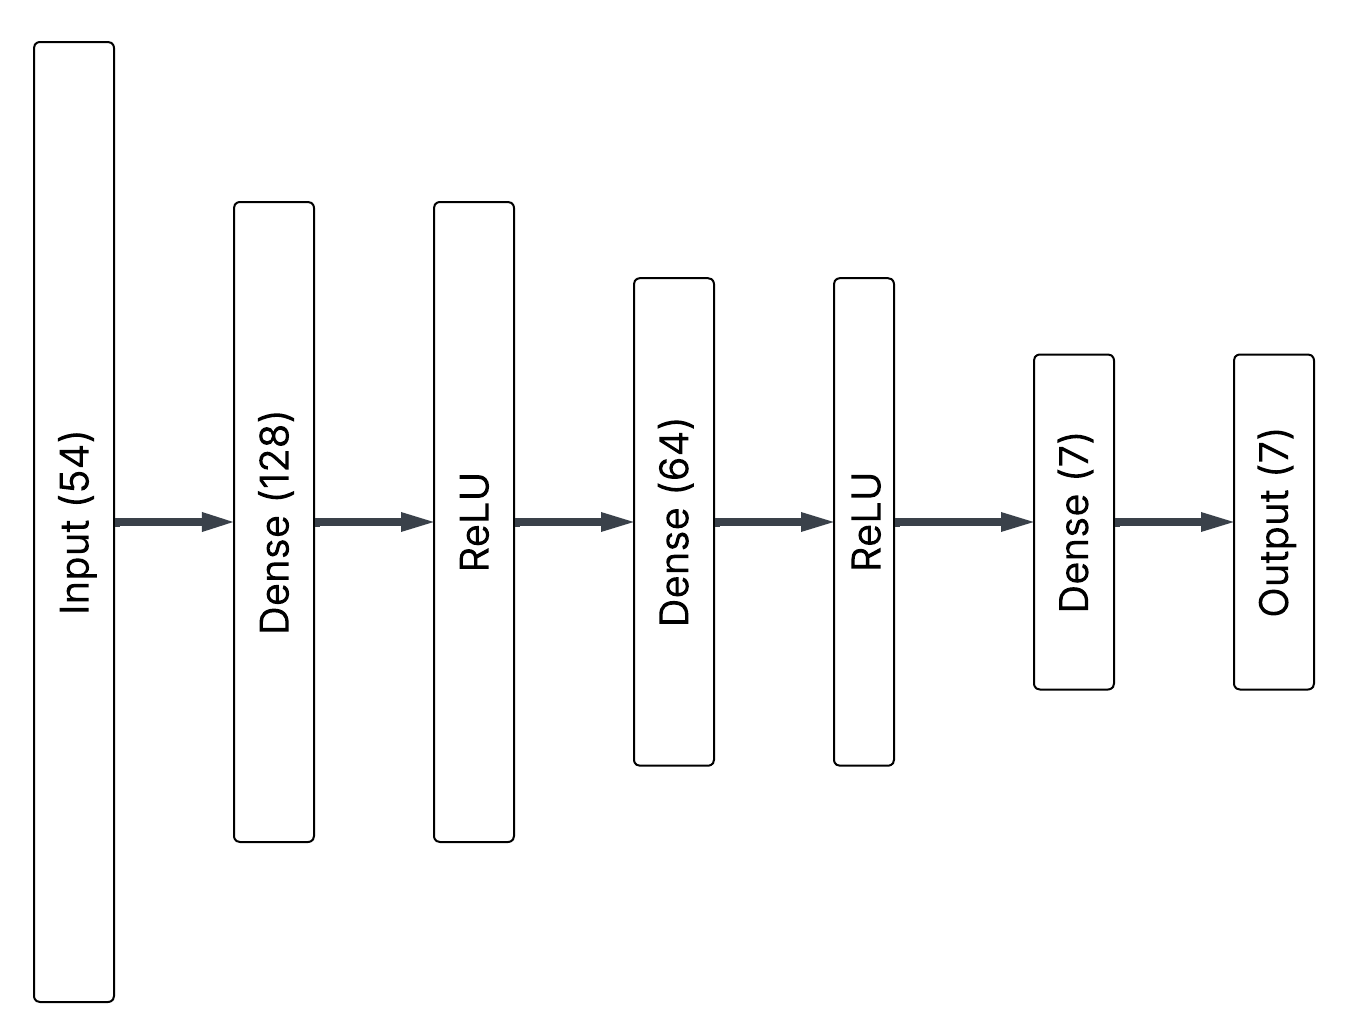
\includegraphics[height=0.28\textheight,width=0.6\textwidth]{Figures/Results/Covertype/Covertype_base_mlp_architecture.png} 
    \captionsetup{justification=centering}  % Ensure the caption is centered
    \caption{base\_mlp architecture for Covertype}
    \label{fig:covertypeMlpBaseArch}
\end{figure}

The training and testing curves in Figures \ref{fig:covertypeTrainCurve} and \ref{fig:covertyoeTestCurve} closely align with theoretical expectations for these models. The results cluster into three distinct tiers: min\_spn and min\_mlp perform at the lowest level, fw\_spn and base\_mlp occupy the middle, and pruned\_spn and max\_spn achieve the highest performance. Within these groupings, SPNs consistently outperform their MLP equivalents. These findings clearly demonstrate that increasing the number of connections in MLP models, as implemented in SPNs, leads to improved model performance and data representation. Moreover, the results underscore that perceptron-based architectures are particularly well-suited to tabular data with well-defined features, as opposed to image data, where individual pixel values carry little standalone meaning.

\begin{figure}[H]
    \centering
    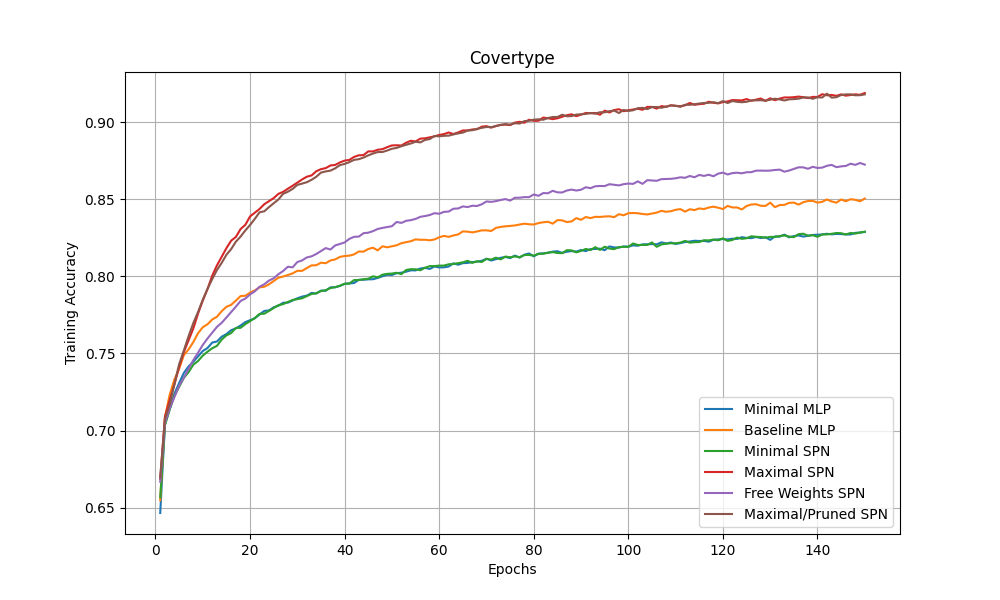
\includegraphics[width=\linewidth]{Figures/Results/Covertype/training_accuracy_plot.png} % first figure itself
    \captionsetup{width=\linewidth}
    \caption{train\_acc vs epochs curve for Covertype}
    \label{fig:covertypeTrainCurve}
\end{figure}

\begin{figure}[H]
    \centering
    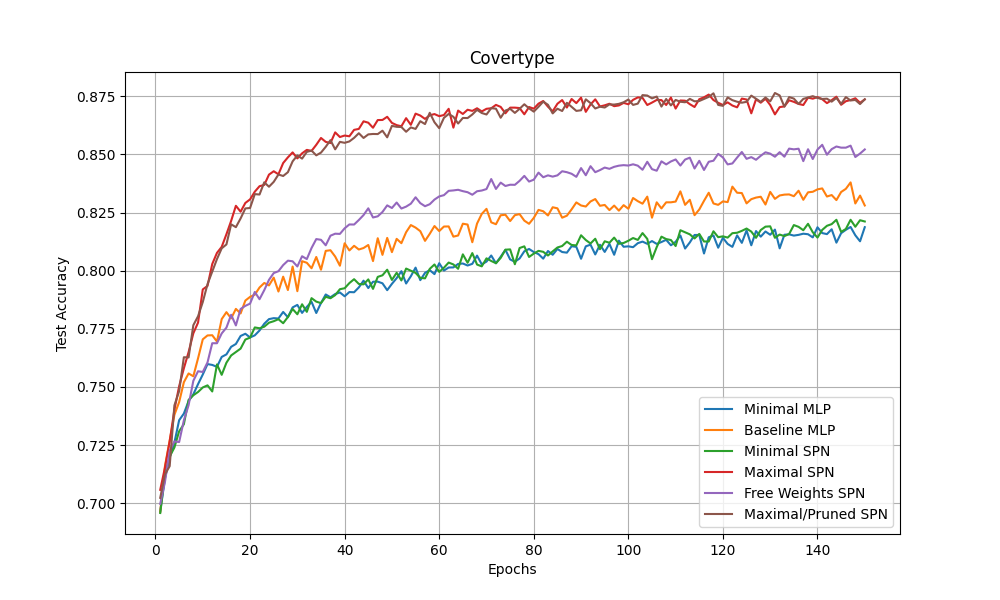
\includegraphics[width=\linewidth]{Figures/Results/Covertype/test_accuracy_plot.png} % second figure itself
    \captionsetup{width=\linewidth}
    \caption{test\_acc vs epochs curve for Covertype}
    \label{fig:covertyoeTestCurve}
\end{figure}

\begin{table}[h!]
    \centering
    \caption{Covertype Dataset results}
    \begin{tabular}{|l|l|l|l|l|l|l|}
    \hline
    \textbf{Model} & \textbf{param\_count} & \textbf{best\_acc} & \textbf{time\_best} & \textbf{train\_eff} & \textbf{auc\_eff} & \textbf{thru\_eff} \\
    \hline
    base\_mlp & 15,751 & 83.79\% & 64.17s & 0.013 & 121.207 & 1.920 \\
    fw\_spn & 20,481 & 85.41\% & 77.07s & 0.011 & 122.954 & 1.554 \\
    min\_mlp & 11,911 & \cellcolor{red!25}81.88\% & \cellcolor{green!25}48.05s & \cellcolor{green!25}0.017 & \cellcolor{red!25}118.777 & \cellcolor{green!25}2.505 \\
    min\_spn & 12,289 & 82.19\% & 50.29s & 0.016 & 118.906 & 2.354 \\
    max\_spn & 30,646 & 87.57\% & \cellcolor{red!25}2430.20s & \cellcolor{red!25}0.0003 & \cellcolor{green!25}127.573 & \cellcolor{red!25}0.042 \\
    pruned\_spn & 30,520 & \cellcolor{green!25}87.64\% & 2082.85s & 0.0004 & 127.413 & 0.055 \\
    \hline
    \end{tabular}
    \label{tab:covertypeResults}
\end{table}

\begin{enumerate}
\item \textbf{Baseline MLP vs. Free Weights SPN}: The fw\_spn model clearly outperforms the base\_mlp in both best accuracy and AUC efficiency, with only a slight reduction in training efficiency. While base\_mlp does achieve better throughput efficiency, this advantage is unlikely to be significant unless the models are deployed in scenarios involving extremely large data volumes.
\item \textbf{Minimal MLP vs. Minimal SPN}: A similar pattern emerges among the minimal models: min\_spn achieves higher accuracy than min\_mlp, with near identical efficiency scores for both. Although min\_mlp boasts the best training and throughput efficiency of all models, its poor accuracy and AUC efficiency make it unusable in a practical scenario.
\item \textbf{Maximal SPN}: The max\_spn model maintains its pattern of poor efficiency but distinguishes itself by achieving a significantly higher peak test accuracy, surpassing even the third-highest accuracy reported on the Covertype dataset leaderboard~\cite{kaggle_covertype_leaderboard}. Additionally, it achieves the best AUC efficiency score, demonstrating that combining maximal layers with extensive connections can lead to rapid and robust performance on this dataset. This approach also highlights the potential upper limit of model performance given the neuron count, making it valuable during the research and development phase for benchmarking what is achievable.
\item \textbf{Pruned SPN}:
\begin{center}  % Centers the table
\begin{tabular}{|l|l|}
\hline
\textbf{Metric} & \textbf{Value} \\
\hline
Layers Before Pruning & 199 \\
Layers After Pruning & 105 \\
Mean Epoch Time Before Pruning & 20.39s \\
Mean Epoch Time After Pruning & 15.66s \\
Pruning Time & 293.63s \\
Pruning Effectiveness & 1.30 \\
\hline
\end{tabular}
\end{center}

The pruning algorithm operates relatively quickly in this case, saving about a minute of training time compared to max\_spn. However, the improvement in throughput is modest and does not significantly enhance overall efficiency. Notably, pruning does lead to a slight increase in peak test accuracy, resulting in the highest test accuracy among all models. This demonstrates that pruning can positively affect not only throughput but also model performance in some instances.

\end{enumerate}

Overall, this dataset most clearly demonstrated the potential of SPNs, with SPN models consistently outperforming their MLP counterparts. The top-performing SPN even achieved results that are highly competitive with state-of-the-art models on this dataset.

\section{Language Domain Results}

For this domain, the data was vectorized using a TF-IDF vectorizer with English stop words removed and a feature size limited to 5,000.

\subsection{Newsgroups 20 Dataset}

\begin{tabular}{@{}ll@{}}
\textbf{Variant} & Simple \\
\textbf{Input Features} & 5000 \\
\textbf{Output Classes} & 20 \\
\textbf{Batch Size} & 64 \\
\textbf{Training Epochs} & 50 \\
\textbf{Training Samples} & 13,192 \\
\textbf{Test Samples} & 5,654 \\
\textbf{Base MLP Dimensions} & $[16,\, 8,\, 20]$ \\
\textbf{Total Neurons} & 44 \\
\end{tabular}

\vspace{2pt}
In early testing, most MLP architectures demonstrated similar performance on this dataset, achieving strong results quickly. This is likely due to the relatively small size of the 20 Newsgroups dataset, which limits the amount of information available for the models to learn. Consequently, to avoid overfitting, a small MLP model was chosen as the baseline.

\begin{figure}[H]
    \centering
    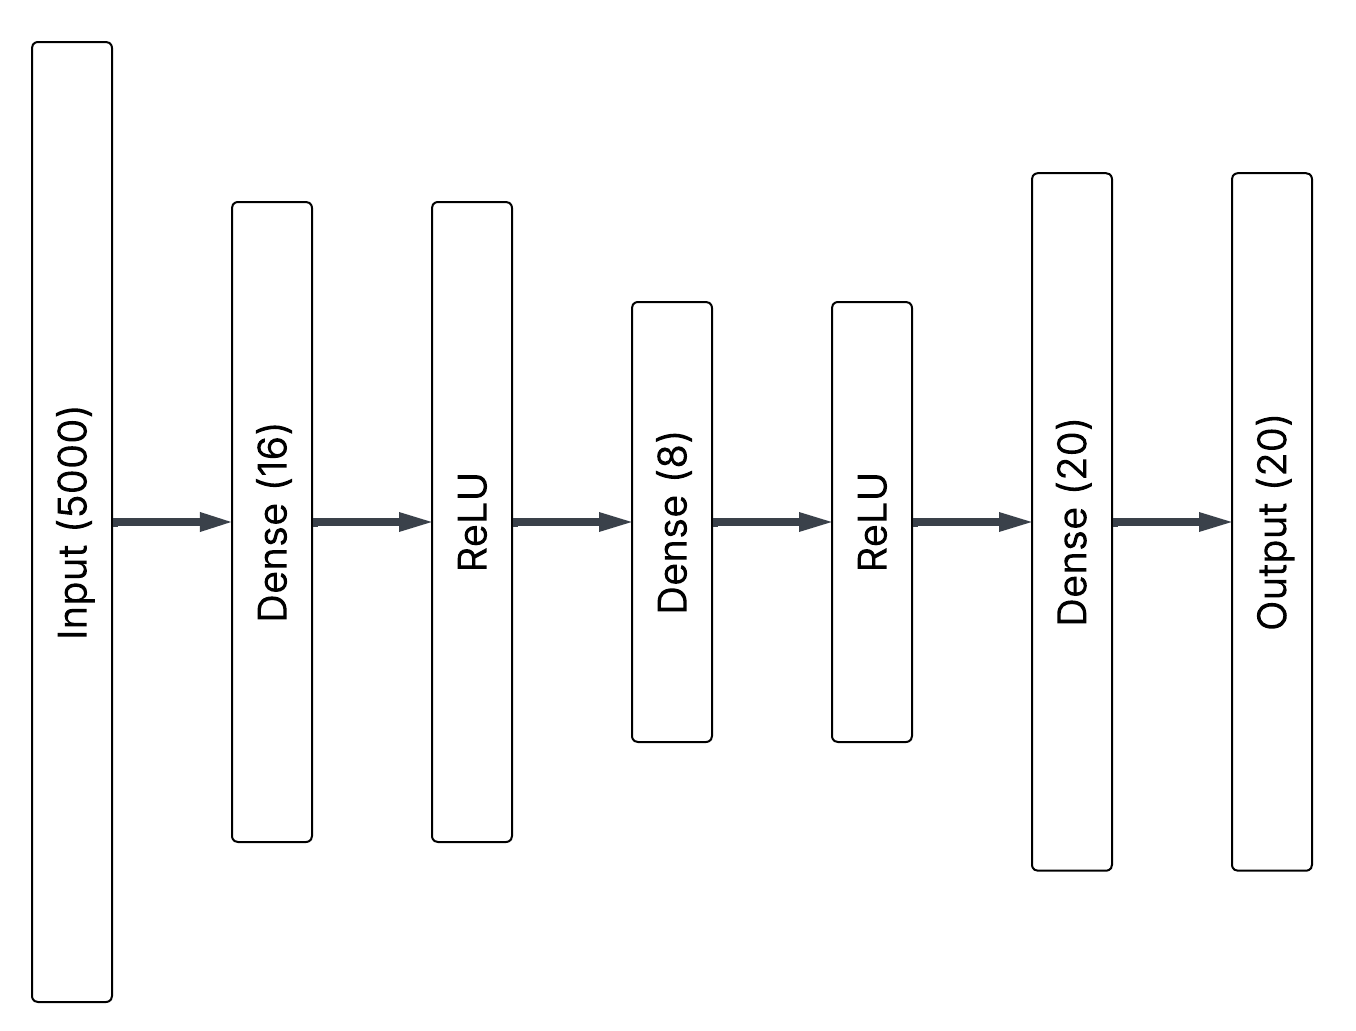
\includegraphics[height=0.28\textheight,width=0.6\textwidth]{Figures/Results/Newsgroups/Newsgroups_base_mlp_architecture.png} 
    \captionsetup{justification=centering}  % Ensure the caption is centered
    \caption{base\_mlp architecture for Newsgroups 20}
    \label{fig:newsgroupsMlpBaseArch}
\end{figure}

The training curves in Figure \ref{fig:newsgroupsTrainCurve} are nearly identical for all models, with the exception of base\_mlp, which converges slightly more slowly. Nevertheless, all models ultimately achieve 100\% training accuracy. In contrast, the test curve in Figure \ref{fig:newsgroupsTestCurve} reveals a clear stratification: the minimal models perform best, followed by fw\_spn, max\_spn, and pruned\_spn, while base\_mlp lags behind. This pattern closely mirrors the results observed in the MNIST experiment.

\begin{figure}[H]
    \centering
    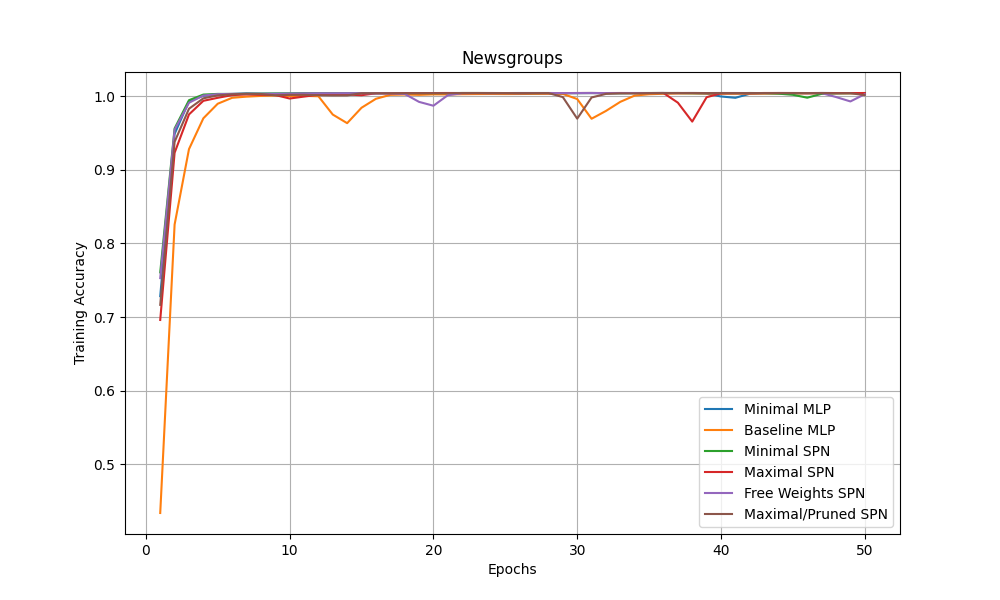
\includegraphics[width=\linewidth]{Figures/Results/Newsgroups/training_accuracy_plot.png} % first figure itself
    \captionsetup{width=\linewidth}
    \caption{train\_acc vs epochs curve for Newsgroups 20}
    \label{fig:newsgroupsTrainCurve}
\end{figure}

\begin{figure}[H]
    \centering
    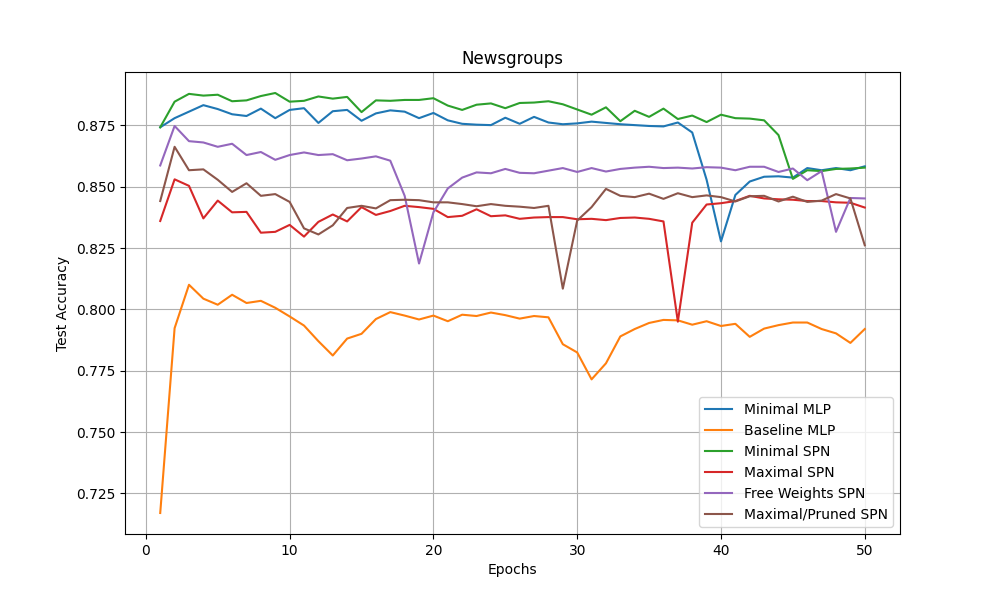
\includegraphics[width=\linewidth]{Figures/Results/Newsgroups/test_accuracy_plot.png} % second figure itself
    \captionsetup{width=\linewidth}
    \caption{test\_acc vs epochs curve for Newsgroups 20}
    \label{fig:newsgroupsTestCurve}
\end{figure}

\begin{table}[h!]
    \centering
    \caption{Newsgroups 20 Dataset results}
    \begin{tabular}{|l|l|l|l|l|l|l|}
    \hline
    \textbf{Model} & \textbf{param\_count} & \textbf{best\_acc} & \textbf{time\_best} & \textbf{train\_eff} & \textbf{auc\_eff} & \textbf{thru\_eff} \\
    \hline
    base\_mlp & 80,332 & \cellcolor{red!25}81.00\% & 0.77s & 1.054 & \cellcolor{red!25}38.869 & 2.938 \\
    fw\_spn & 220,652 & 87.48\% & \cellcolor{green!25}0.64s & \cellcolor{green!25}1.371 & 41.990 & 2.757 \\
    min\_mlp & 120,524 & 88.33\% & 0.91s & 0.967 & 42.720 & 3.937 \\
    min\_spn & 220,524 & \cellcolor{green!25}88.82\% & 2.14s & 0.415 & \cellcolor{green!25}43.105 & \cellcolor{green!25}4.270 \\
    max\_spn & 220,990 & 85.30\% & \cellcolor{red!25}7.99s & \cellcolor{red!25}0.107 & 41.103 & \cellcolor{red!25}0.217 \\
    pruned\_spn & 220,834 & 86.63\% & 1.39s & 0.625 & 41.356 & 1.265 \\
    \hline
    \end{tabular}
    \label{tab:newsgroupsResults}
\end{table}

\begin{enumerate}
\item \textbf{Baseline MLP vs. Free Weights SPN}: This experiment exhibited the largest gap in test accuracy between base\_mlp and the other models, as well as one of the most pronounced differences in parameter count. These findings provide strong evidence that increasing the number of connections can substantially improve performance on certain types of data. Notably, fw\_spn not only outperformed base\_mlp by a significant margin but also achieved the highest training efficiency in this test, making it particularly well-suited for research applications.
\item \textbf{Minimal MLP vs. Minimal SPN}: Surprisingly, the minimal models achieved the highest test accuracy in this experiment. Which suggests that having more layers might be disadvantageous for this kind of data. The min\_spn model, in particular, attained the third-highest test accuracy on the 20 Newsgroups leaderboard~\cite{pwc_20newsgroups_leaderboard}. Combined with its top scores in both AUC efficiency and throughput efficiency, min\_spn stands out as the best-performing model for this dataset among all those tested, making it the clear choice for practical applications.

Min\_mlp also performed well, ranking second in AUC efficiency, throughput efficiency, and test accuracy, but with min\_spn’s outstanding results, the competition was decisively one-sided.
\item \textbf{Maximal SPN}: Unexpectedly, max\_spn produced the second lowest test accuracy while continuing its trend of poor efficiency. This outcome reinforces that increasing model depth does not benefit this type of data; in fact, simpler models might be better suited to capturing the information present in vectorized text.
\item \textbf{Pruned SPN}:
\begin{center}  % Centers the table
\begin{tabular}{|l|l|}
\hline
\textbf{Metric} & \textbf{Value} \\
\hline
Layers Before Pruning & 24 \\
Layers After Pruning & 7 \\
Mean Epoch Time Before Pruning & 3.87s \\
Mean Epoch Time After Pruning & 0.69s \\
Pruning Time & 70.55s \\
Pruning Effectiveness & 5.61 \\
\hline
\end{tabular}
\end{center}

While pruned\_spn outperforms max\_spn across all metrics, its pruning time is nearly ten times longer than the time required for max\_spn to reach its best accuracy. Given the already poor performance of max\_spn, this excessive pruning time renders the process impractical.

\end{enumerate}

Overall, this dataset proved to be the most interesting so far. It was the first instance where the minimal models outperformed their more complex, deeper counterparts. At the same time, the benefits of increased connectivity were clearly demonstrated, with both min\_spn and fw\_spn surpassing their respective MLP counterparts. These results suggest that SPNs may not only enhance performance but also provide insights into the optimal layer complexity and connection density needed for a given dataset.

\subsection{IMDB Reviews Dataset}

\begin{tabular}{@{}ll@{}}
\textbf{Variant} & Complex \\
\textbf{Input Features} & 5000 \\
\textbf{Output Classes} & 2 \\
\textbf{Batch Size} & 32 \\
\textbf{Training Epochs} & 50 \\
\textbf{Training Samples} & 25,000 \\
\textbf{Test Samples} & 25,000 \\
\textbf{Base MLP Dimensions} & $[64,\, 32,\, 2]$ \\
\textbf{Total Neurons} & 96 \\
\end{tabular}

\vspace{2pt}
Preliminary tests on this dataset revealed overfitting issues similar to those observed with CIFAR-10, while also demonstrating that models achieved strong performance early in training, as seen with 20 Newsgroups. Despite this, the best test accuracies were above 80\%, leaving considerable room for improvement through SPNs. Therefore, a mid-sized, three-layer MLP was selected as the baseline for further comparison.

\begin{figure}[H]
    \centering
    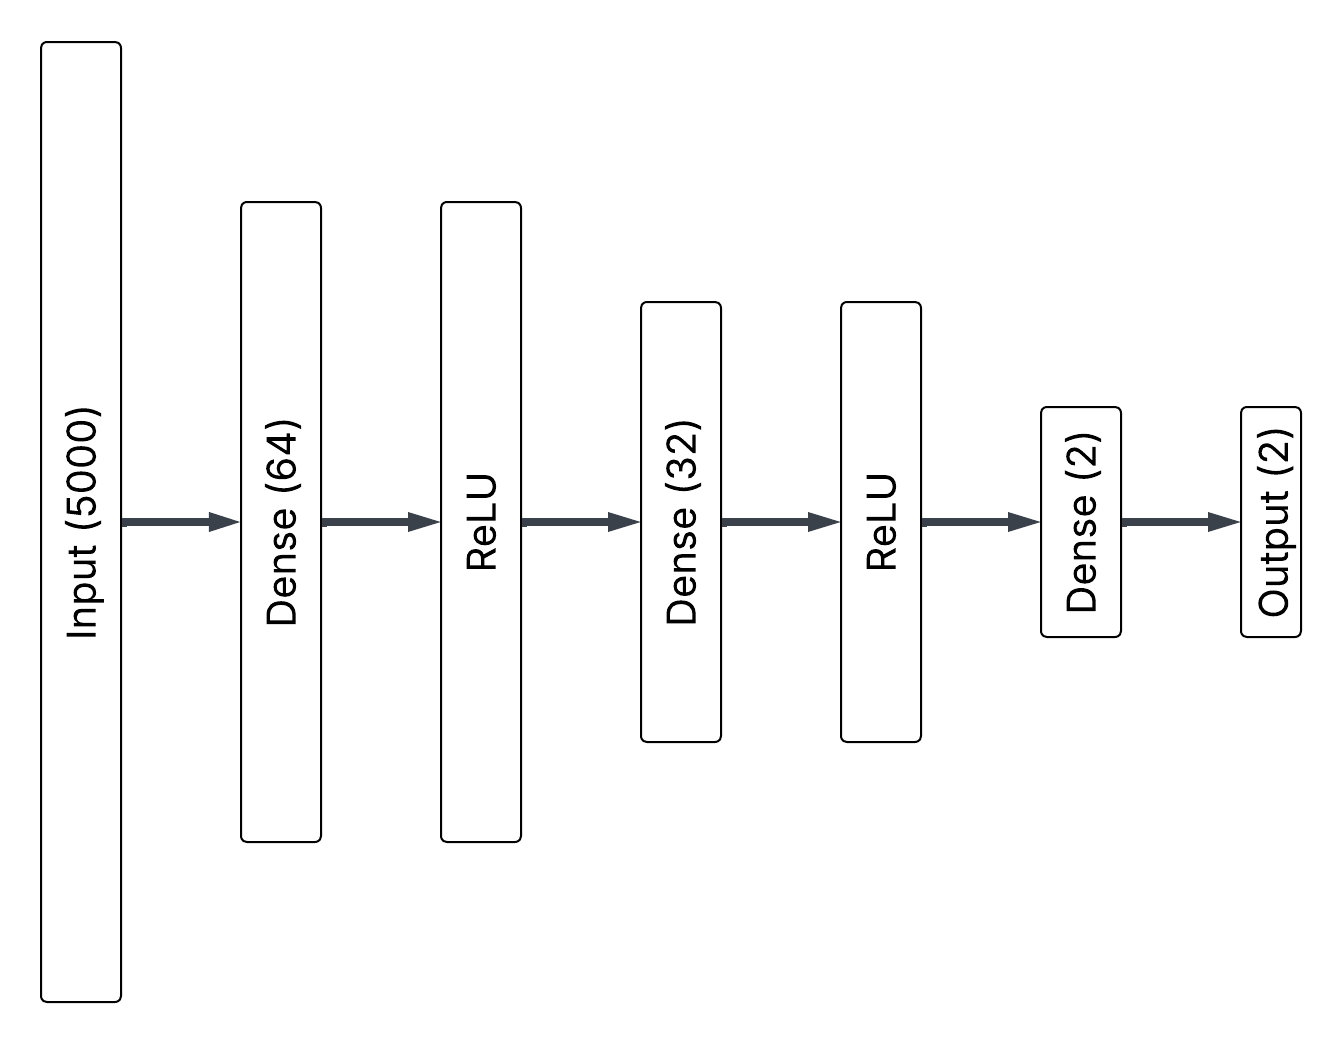
\includegraphics[height=0.28\textheight,width=0.6\textwidth]{Figures/Results/IMDB/IMDB_base_mlp_architecture.png} 
    \captionsetup{justification=centering}  % Ensure the caption is centered
    \caption{base\_mlp architecture for IMDB Reviews}
    \label{fig:imdbMlpBaseArch}
\end{figure}

The training curve in Figure \ref{fig:imdbTrainCurve} closely resembles that of the Newsgroups dataset in Figure \ref{fig:newsgroupsTrainCurve}. However, the test curve in Figure \ref{fig:imdbTestCurve} reveals a steady decline in accuracy as training progresses, indicating pronounced overfitting. This suggests that perceptron-based models may struggle with more complex text tasks, such as sentiment analysis, compared to simpler classification problems.

\begin{figure}[H]
    \centering
    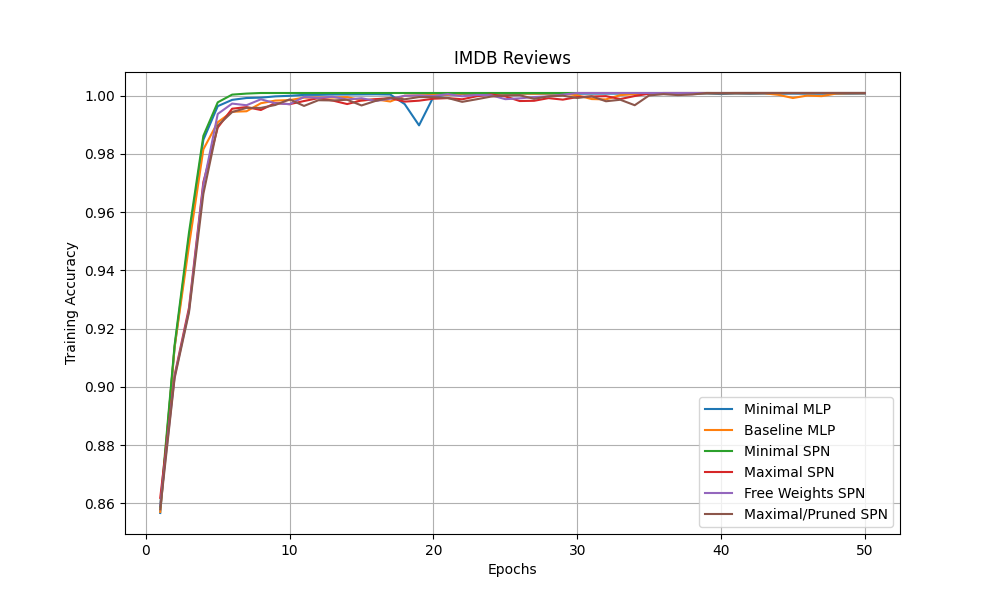
\includegraphics[width=\linewidth]{Figures/Results/IMDB/training_accuracy_plot.png} % first figure itself
    \captionsetup{width=\linewidth}
    \caption{train\_acc vs epochs curve for IMDB Reviews}
    \label{fig:imdbTrainCurve}
\end{figure}

\begin{figure}[H]
    \centering
    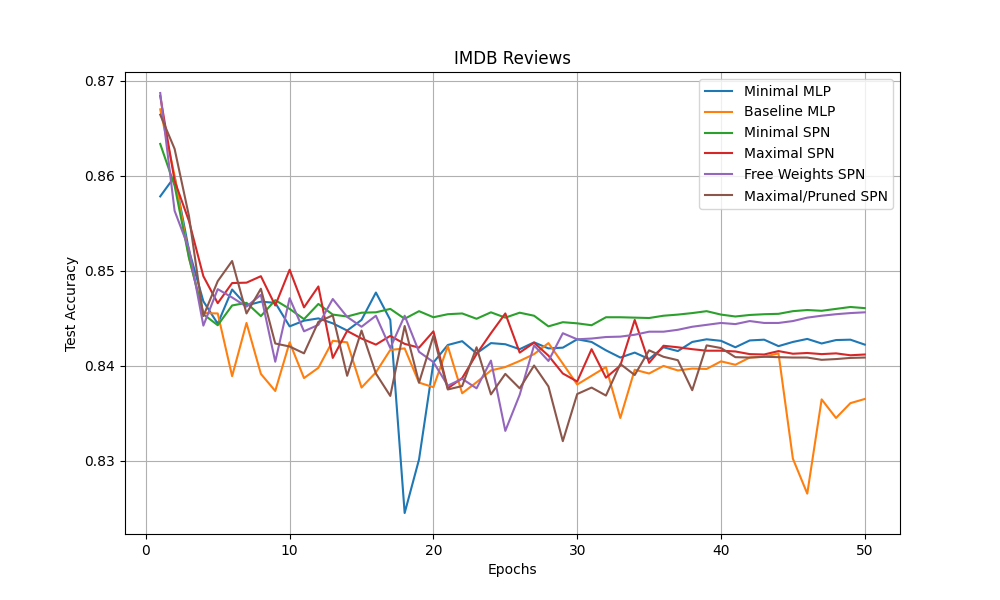
\includegraphics[width=\linewidth]{Figures/Results/IMDB/test_accuracy_plot.png} % second figure itself
    \captionsetup{width=\linewidth}
    \caption{test\_acc vs epochs curve for IMDB Reviews}
    \label{fig:imdbTestCurve}
\end{figure}

\begin{table}[h!]
    \centering
    \caption{IMDB Reviews Dataset results}
    \begin{tabular}{|l|l|l|l|l|l|l|}
    \hline
    \textbf{Model} & \textbf{param\_count} & \textbf{best\_acc} & \textbf{time\_best} & \textbf{train\_eff} & \textbf{auc\_eff} & \textbf{thru\_eff} \\
    \hline
    base\_mlp & 322,210 & 86.70\% & 1.09s & 0.792 & \cellcolor{red!25}41.175 & 0.787 \\
    fw\_spn & 492,338 & \cellcolor{green!25}86.87\% & 1.53s & 0.569 & 41.360 & 0.550 \\
    min\_mlp & 480,290 & \cellcolor{red!25}85.99\% & 1.85s & 0.466 & 41.319 & \cellcolor{green!25}1.009 \\
    min\_spn & 490,290 & 86.34\% & \cellcolor{green!25}0.90s & \cellcolor{green!25}0.955 & \cellcolor{green!25}41.455 & 0.954 \\
    max\_spn & 494,851 & 86.84\% & \cellcolor{red!25}35.29s & \cellcolor{red!25}0.025 & 41.340 & \cellcolor{red!25}0.025 \\
    pruned\_spn & 494,810 & 86.64\% & 27.01s & 0.032 & 41.255 & 0.032 \\
    \hline
    \end{tabular}
    \label{tab:imdbResults}
\end{table}

\begin{enumerate}
\item \textbf{Baseline MLP vs. Free Weights SPN}: Since all models achieved nearly identical best test accuracy, it is difficult to conclude that increasing connectivity or layers in MLPs through SPNs offers any significant advantage. Although fw\_spn obtained the highest test accuracy, it lagged behind base\_mlp in both training and throughput efficiency. While base\_mlp had the lowest AUC efficiency, the difference was marginal compared to the other models. Given the similar overall performance, there appears to be little benefit to sacrificing efficiency for such minimal gains.
\item \textbf{Minimal MLP vs. Minimal SPN}: The minimal models followed a similar pattern. While min\_spn was the most efficient overall, min\_mlp achieved slightly higher throughput efficiency, and min\_spn attained marginally better test accuracy.
\item \textbf{Maximal SPN}: While max\_mlp achieved the second-highest test accuracy in this task, the absence of any substantial improvement indicates that simply adding layers or complexity is insufficient. Instead, these results highlight the limitations of perceptron-based models for this type of task, suggesting that the underlying architecture itself is the primary constraint.
\item \textbf{Pruned SPN}:
\begin{center}  % Centers the table
\begin{tabular}{|l|l|}
\hline
\textbf{Metric} & \textbf{Value} \\
\hline
Layers Before Pruning & 96 \\
Layers After Pruning & 63 \\
Mean Epoch Time Before Pruning & 35.20s \\
Mean Epoch Time After Pruning & 27.01s \\
Pruning Time & 253.58s \\
Pruning Effectiveness & 1.30 \\
\hline
\end{tabular}
\end{center}

While pruned\_spn offered a modest improvement over max\_mlp in terms of performance, the substantial pruning time rendered it largely impractical.

\end{enumerate}

Overall, SPNs showed a slight advantage over MLPs in this task, but all the models performed significantly worse than the top models on the IMDb Reviews leaderboard~\cite{pwc_imdb_sota}. These results further suggest that perceptron-based models are not well-suited for complex data tasks like sentiment analysis.

\section{Discussion}

This section seeks to answer the research questions posed in the introduction using the findings from the experimental results.

\subsection*{RQ1: Does increasing connection density in SPNs, while keeping the layer count and design identical to MLPs, lead to better model performance?}

Across the majority of experiments, especially for the MNIST image dataset and both tabular datasets, SPNs with increased connection density clearly outperformed traditional MLPs with the same number of layers and neurons. In Table~\ref{tab:mnistResults} and Table~\ref{tab:covertypeResults}, fw\_spn consistently achieved higher test accuracy than base\_mlp, confirming that enhanced connectivity can yield better model performance. This effect was strongest in structured datasets where feature relationships are important and more easily captured with additional internal connections.

\subsection*{RQ2: Does removing connectivity restrictions in MLP architectures (allowing arbitrary neuron-to-neuron connections) enhance the network’s learning capability or representational power?}

The results affirm that lifting connectivity restrictions enhances both representational capacity and learning ability. In both simple and complex tabular datasets, SPNs consistently demonstrated better performance, as indicated by higher best test accuracy and area under curve efficiency. However, in highly complex domains such as CIFAR-10 and IMDB Reviews, the representational advantage of SPNs was limited by the fundamental capabilities of perceptron-based models, which struggle to capture spatial or semantic relationships lost during input flattening or vectorization. Thus, while enhanced connectivity is powerful, its effectiveness is domain-dependent.

\subsection*{RQ3: Can SPNs with fewer layers but higher connection density match or exceed the performance of deeper MLPs, thereby improving throughput efficiency and reducing training times?}

Experiments with minimal models show that shallow, densely connected networks can often match or surpass deeper MLPs, especially on tabular and certain text datasets (e.g., Newsgroups 20). For instance, Table~\ref{tab:newsgroupsResults} demonstrates that min\_spn achieved both the highest test accuracy and best efficiency scores, while maintaining a slight edge over min\_mlp in test accuracy across most tasks. This supports the view that increasing connection density can compensate for network depth, resulting in more efficient architectures without sacrificing performance.

\subsection*{RQ4: How do SPNs compare to MLPs in terms of training time, computational efficiency, memory usage, and predictive accuracy across a range of datasets and tasks?}

SPNs generally require more memory due to their larger parameter count, as seen in all summary tables. However, their training efficiency and throughput efficiency were often on par with, or better than, MLPs, especially in the tabular and simple datasets. Notably, pruned SPNs demonstrated that computational efficiency can be recovered through targeted pruning, reducing both training time and memory usage while preserving accuracy (see Tables~\ref{tab:mnistResults}, \ref{tab:covertypeResults}). On complex image and language tasks, neither MLPs nor SPNs could match the specialized models (CNNs, ViTs, Transformers), and the efficiency benefits of SPNs were less pronounced.

\subsection*{RQ5: Does the increased architectural flexibility of SPNs improve their ability to generalize across diverse datasets and tasks compared to standard MLPs?}

The experimental results show that SPNs' flexibility improves generalization in many settings, particularly for tabular and structured datasets. The ability to learn from more complex feature interactions enables SPNs to adapt to different data distributions, resulting in more robust performance across tasks. However, for highly unstructured or semantically complex tasks, such as image classification in CIFAR-10 or sentiment analysis in IMDB Reviews, the generalization advantage of SPNs diminishes, and specialized architectures remain superior.

\subsection*{RQ6: After maximizing connections in SPNs, can pruning strategies maintain high predictive performance while significantly improving computational efficiency and training time?}

Pruning strategies applied to maximal SPNs were largely successful in reducing computational overhead without substantially sacrificing predictive accuracy. For example, in the MNIST and Covertype experiments, pruned SPNs maintained or even slightly improved peak test accuracy while reducing mean epoch time (see corresponding metrics tables). However, the practical benefit was sometimes offset by the additional time required for the pruning process itself, indicating that more efficient pruning algorithms could further enhance the value of this approach.